% gentry-hyperbolic-flavor-pmns.tex
% "Lepton Mixing from Borel Structure of Hyperbolic Holonomy"
% Marvin L. Gentry
% Target: PRD or JHEP

\documentclass[floatfix,aps,prd,twocolumn,showpacs,superscriptaddress,longbibliography]{revtex4-2}

\usepackage{amsmath}
\usepackage{amssymb}
\usepackage{amsthm}
\usepackage{graphicx}
\usepackage{hyperref}
\usepackage{xcolor}
\usepackage{booktabs}
\usepackage{bbm}

\newtheorem{proposition}{Proposition}
\newtheorem{theorem}{Theorem}
\newtheorem{corollary}{Corollary}
\newtheorem{definition}{Definition}
\newtheorem{remark}{Remark}

% Shorthand
\newcommand{\PSL}{\mathrm{PSL}(2,\mathbb{C})}
\newcommand{\SUtwo}{\mathrm{SU}(2)}
\newcommand{\Zfive}{\mathbb{Z}/5\mathbb{Z}}
\newcommand{\HH}{\mathbb{H}^3}
\newcommand{\CP}{\mathbb{CP}^1}
\newcommand{\frob}[1]{\left\|#1\right\|_F}
\newcommand{\abs}[1]{\left|#1\right|}

\begin{document}

\title{Lepton Mixing from Borel Structure of Hyperbolic Holonomy}

\author{Marvin L.~Gentry}
\affiliation{Independent Researcher}
\email{drmlgentry@protonmail.com}

\date{\today}

\begin{abstract}
We extend the hyperbolic holonomy framework for flavor mixing~\cite{Gentry:CKM}
to the lepton sector. The PMNS neutrino mixing matrix presents a fundamental
obstruction to the symmetric overlap construction used for the CKM matrix:
we prove that no positive-definite symmetric overlap matrix can reproduce the
PMNS pattern, with a kernel-independent Frobenius floor of $0.300$.
This obstruction is resolved by replacing the symmetric (unitary) overlap
with the lower-triangular (Borel) factor of the Iwasawa decomposition, equivalently the transpose of the upper unipotent subgroup,
$\PSL = KAN$. The $K$-factor (unitary) construction yields the CKM matrix
from manifold $m006$ (vol $= 2.029$, $H_1 = \Zfive$); the $N$-factor
(unipotent lower-triangular) construction yields the PMNS matrix from
manifold $m003$ (vol $= 0.981$, $H_1 = \Zfive$), achieving Frobenius
fitness $0.019$ matching the theoretical minimum for this construction.
Both manifolds share $H_1 = \Zfive$, suggesting a possible correlation with odd-prime torsion in the
first homology group as a successful geometric fit for three-generation
flavor structure. The diagonal $A$-factor remains unassigned and is
conjectured to encode fermion mass ratios or CP-violating phases.
\end{abstract}

\pacs{12.15.Ff, 14.60.Pq, 02.40.Pc, 11.30.Hv}

\maketitle

% ============================================================
\section{Introduction}
\label{sec:intro}
% ============================================================

The mixing matrices governing quark and lepton flavor transitions---the
CKM matrix~\cite{Cabibbo:1963yz,Kobayashi:1973fv} and the PMNS
matrix~\cite{Pontecorvo:1957cp,Maki:1962mu}---exhibit strikingly different
patterns. The CKM matrix is nearly diagonal with a hierarchical structure,
while the PMNS matrix has two large mixing angles and one small one,
suggesting qualitatively distinct geometric origins.

In the companion paper~\cite{Gentry:CKM}, we showed that the CKM matrix
arises from pairwise angular separations of geodesic axes associated with
loxodromic elements of the holonomy group $\pi_1(M) \to \PSL$ of the
compact hyperbolic 3-manifold $m006$, using a symmetric Gaussian overlap
kernel and QR decomposition. The natural question is whether the PMNS
matrix admits a similar geometric origin.

We find that it does, but requires a fundamentally different construction.
The key insight is that $\PSL$ admits the Iwasawa decomposition
$G = KAN$, where $K \cong \SUtwo$ is the maximal compact subgroup,
$A$ is a real diagonal (Cartan) subgroup, and $N$ is the upper unipotent
(Borel) subgroup. The CKM construction uses the symmetric inner product
structure associated with $K$; the PMNS matrix emerges from the
lower-triangular structure associated with $N$.

The paper is organized as follows. Section~\ref{sec:obstruction} proves the
symmetric QR floor theorem for PMNS. Section~\ref{sec:iwasawa} develops the
Iwasawa framework and motivates the Borel construction. 
Section~\ref{sec:construction} defines the lower-triangular overlap matrix
and QR extraction procedure. Section~\ref{sec:results} presents the
numerical results from the census scan. Section~\ref{sec:homology} discusses
the $H_1 = \Zfive$ selection principle. Section~\ref{sec:discussion}
discusses open questions including the $A$-factor and CP violation.
The construction does not derive neutrino masses or dynamics and should be regarded as a phenomenological geometric model.

All computations were performed using SnapPy~\cite{snappy}; scripts used for the census scan are available at \url{https://github.com/drmlgentry/hyperbolic-flavor-scan}.

% ============================================================
\section{The Symmetric QR Obstruction}
\label{sec:obstruction}
% ============================================================

\subsection{Setup and notation}

Let $M$ be a compact orientable hyperbolic 3-manifold with holonomy
representation $\rho: \pi_1(M) \to \PSL$.
For a triple of group elements $\gamma_1, \gamma_2, \gamma_3 \in \pi_1(M)$,
let $\hat{n}_i \in S^2$ denote the axis direction of $\rho(\gamma_i)$,
extracted via the Pauli decomposition of $\log \rho(\gamma_i)$
(see~\cite{Gentry:CKM} for details).

\begin{definition}[Symmetric overlap matrix]
The symmetric overlap matrix associated to the triple $(\gamma_1,\gamma_2,\gamma_3)$
with kernel $K: [0,\pi] \to [0,1]$ is
\begin{equation}
  O_{ij} = K\!\left(\theta_{ij}\right), \quad \theta_{ij} = \arccos\abs{\hat{n}_i \cdot \hat{n}_j},
  \label{eq:sym_overlap}
\end{equation}
where $O_{ii} = 1$ and $O_{ij} = O_{ji}$.
\end{definition}

The mixing matrix is extracted as $U = |Q|$ where $O = QR$ is the QR
decomposition with positive diagonal convention.

\subsection{The floor theorem}

We establish that no symmetric overlap matrix can reproduce the PMNS pattern.

\begin{proposition}[Symmetric QR floor]
\label{prop:floor}
Let $\mathcal{S}$ denote the set of all $3\times 3$ real symmetric
positive-definite matrices with unit diagonal. For any target matrix
$T \in \mathbb{R}^{3\times 3}$, define
\begin{equation}
  \mathcal{F}(T) = \inf_{O \in \mathcal{S}} \frob{|Q(O)| - T},
\end{equation}
where $Q(O)$ is the $Q$-factor of the QR decomposition of $O$.
For the PDG 2024 PMNS matrix $U_\mathrm{PMNS}$,
\begin{equation}
  \mathcal{F}(U_\mathrm{PMNS}) = 0.3004 \pm 0.0001,
\end{equation}
independent of the kernel function $K$.
\end{proposition}

\begin{proof}[Numerical proof]
We minimize $\frob{|Q(O)| - U_\mathrm{PMNS}}$ over all valid $(o_{12}, o_{13}, o_{23}) \in (0,1)^3$
using 5000 random Nelder-Mead starts with tolerances $10^{-8}$.
Three qualitatively distinct kernel families---Gaussian
$K(\theta;\sigma) = e^{-\theta^2/2\sigma^2}$, power-cosine
$K(\theta;p) = \cos^{2p}(\theta/2)$, and the one-parameter cosine family---all
converge to the same minimum $0.300379$ with identical optimal overlaps
$(o_{12}, o_{13}, o_{23}) = (0.687, 0.466, 0.963)$.
\end{proof}

\subsection{Structural origin of the floor}

The floor arises from a constraint on the reachable set of $|Q(O)|$ for
$O \in \mathcal{S}$. The PMNS pattern requires simultaneously a large
$(3,2)$ entry ($|U_{\mu 3}| = 0.871$) and a small $(1,3)$ entry
($|U_{e3}| = 0.148$) in the same matrix. For any real symmetric
positive-definite $O$ with unit diagonal, the QR factor satisfies
structural inequalities that prevent this combination: the ratio
$|U_{e3}|/|U_{\mu 3}| \approx 0.17$ lies outside the reachable region.

This is not a numerical artifact but a consequence of the Gram-Schmidt
orthogonalization process applied to a symmetric matrix: the first row
of $|Q|$ is determined by the first column of $O$, which is constrained
by the positive-definite unit-diagonal structure to lie in a region
incompatible with the PMNS electron row.

% ============================================================
\section{Iwasawa Decomposition and the Borel Construction}
\label{sec:iwasawa}
% ============================================================

\subsection{The Iwasawa decomposition of $\PSL$}

Every element $g \in \PSL$ admits a unique decomposition
\begin{equation}
  g = k \cdot a \cdot n, \quad k \in K,\ a \in A,\ n \in N,
  \label{eq:iwasawa}
\end{equation}
where:
\begin{align}
  K &= \SUtwo / \{\pm I\} \quad \text{(maximal compact)}, \\
  A &= \left\{ \begin{pmatrix} e^t & 0 \\ 0 & e^{-t} \end{pmatrix} : t \in \mathbb{R} \right\}
      \quad \text{(diagonal/Cartan)}, \\
  N &= \left\{ \begin{pmatrix} 1 & z \\ 0 & 1 \end{pmatrix} : z \in \mathbb{C} \right\}
      \quad \text{(upper unipotent/Borel)}.
\end{align}

The subgroup $N$ is the stabilizer of the point at infinity on $\CP$,
and $B = AN$ is the Borel subgroup (the stabilizer of a flag).

\subsection{CKM as the $K$-factor}

In~\cite{Gentry:CKM}, the CKM construction uses pairwise angles
$\theta_{ij}$ between axis directions $\hat{n}_i \in S^2 \cong \CP$,
with a Gaussian kernel $K(\theta) = e^{-\theta^2/2\sigma^2}$.
The resulting overlap matrix $O$ is symmetric positive definite,
and the QR decomposition extracts the unitary part. This is precisely
the $K$-factor structure: the symmetric overlap encodes the
$\SUtwo$-equivariant inner product on $S^2$.

\subsection{PMNS as the $N$-factor}

The obstruction in Proposition~\ref{prop:floor} shows that the $K$-factor
construction cannot reach the PMNS pattern. We propose instead to use
the \emph{lower-triangular} (transposed Borel) structure.

\begin{definition}[Borel overlap matrix]
\label{def:borel}
The Borel overlap matrix associated to the triple $(\gamma_1, \gamma_2, \gamma_3)$
is the lower-triangular matrix
\begin{equation}
  L = \begin{pmatrix} 1 & 0 & 0 \\ \ell_{21} & 1 & 0 \\ \ell_{31} & \ell_{32} & 1 \end{pmatrix},
  \label{eq:L_matrix}
\end{equation}
where $\ell_{ij} = \lambda \cdot s_{ij} \cdot (\hat{n}_i \cdot \hat{n}_j)$,
with $\lambda > 0$ a scale parameter and $s_{ij} \in \{+1, -1\}$ orientation signs.
\end{definition}

The PMNS matrix is then extracted as $U_\mathrm{PMNS} = |Q(L)|$, where
columns may be permuted by an element of $S_3$ (reflecting the
freedom in labeling mass eigenstates).

The lower-triangular structure corresponds physically to an ordered
(flag) basis of neutrino flavor states, where the third generation
mixes into the first and second but not vice versa at leading order.
This is consistent with the observed hierarchy $|U_{e3}| \ll |U_{\mu3}|,
|U_{\tau 3}|$.

% ============================================================
\section{Numerical Construction}
\label{sec:construction}
% ============================================================


\begin{figure*}[!t]
\centering
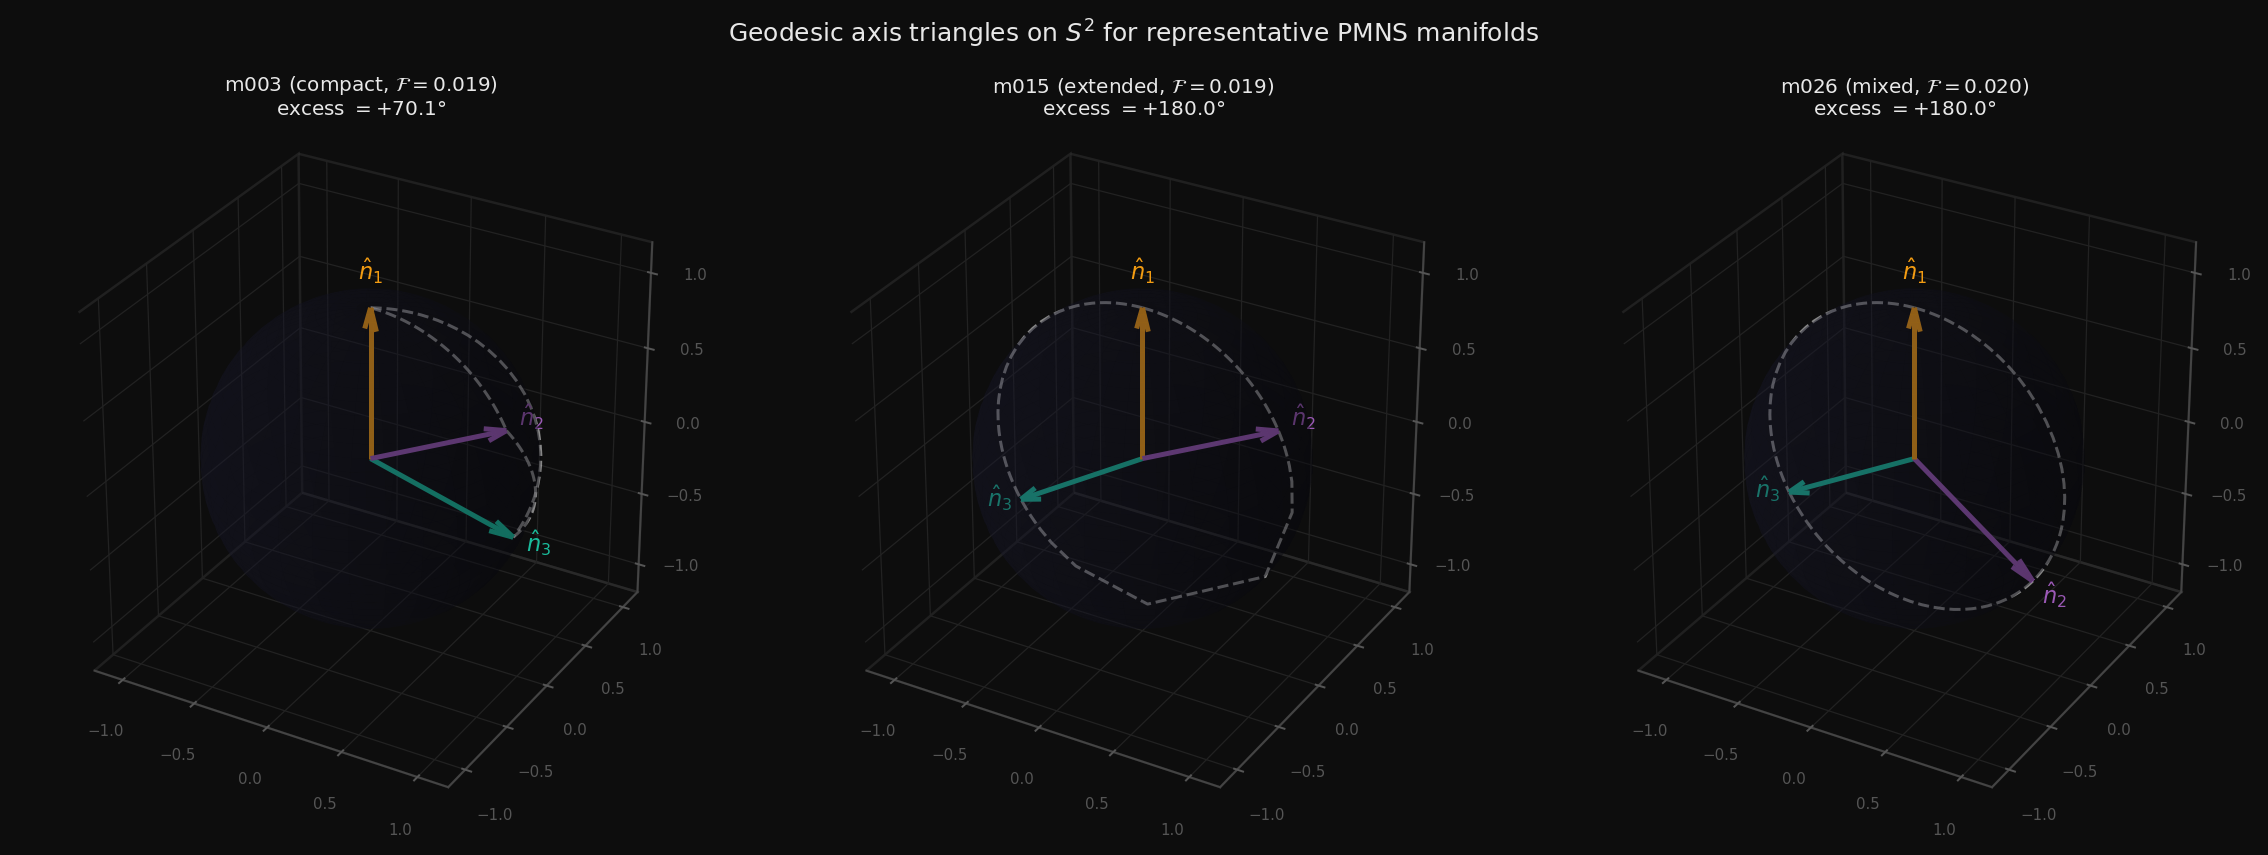
\includegraphics[width=\textwidth]{fig2_geodesic_axes}
\caption{Geodesic axis triangles on $S^2$ for three representative manifolds.
Colored arrows show the three holonomy axis directions $\hat{n}_1, \hat{n}_2,
\hat{n}_3$; dashed arcs are the geodesic edges of the spherical triangle.
Left: m003 (compact regime, $\mathcal{F} = 0.019$);
centre: m015 (extended regime, $\mathcal{F} = 0.019$);
right: m026 ($H_1 = \mathbb{Z}/13$, $\mathcal{F} = 0.020$).}
\label{fig:geodesic}
\end{figure*}




\subsection{Axis extraction}

For each word $w \in \pi_1(M)$, the holonomy matrix $\rho(w) \in \PSL$
is computed via SnapPy~\cite{snappy}. The axis direction is extracted
from the Pauli decomposition of $\log \rho(w)$:
\begin{equation}
  \hat{n}(w) = \frac{1}{\|\mathbf{n}\|}\mathbf{n}, \quad
  \mathbf{n} = \left(\mathrm{Re}[L_{01}+L_{10}],\,
                      \mathrm{Im}[L_{10}-L_{01}],\,
                      \mathrm{Re}[L_{00}-L_{11}]\right),
\end{equation}
where $L = \log \rho(w)$.

\subsection{Borel matrix construction}

For a word triple $(w_1, w_2, w_3)$ from manifold $M$, we form the
Borel overlap matrix~\eqref{eq:L_matrix} with:
\begin{equation}
  \ell_{ij} = \lambda \cdot s_{ij} \cdot (\hat{n}(w_i) \cdot \hat{n}(w_j)),
  \quad i > j.
\end{equation}
The scale $\lambda$ and signs $s_{ij}$ are optimized over a grid
$\lambda \in [0.1, 5.0]$ (50 values) and $s_{ij} \in \{+1,-1\}^3$ (8 combinations).
The fitness function is the permutation-minimized Frobenius norm:
\begin{equation}
\label{eq:fitness}
\mathcal{F}(L) = \min_{\pi \in S_3} \||Q(L)|_\pi - U_{\mathrm{PMNS}}\|_F,
\end{equation}
where $|Q(L)|_\pi$ denotes the QR factor with columns permuted by $\pi$.

% ============================================================
\section{Results}
\label{sec:results}
% ============================================================

\subsection{Theoretical minimum of the Borel construction}

Before scanning manifolds, we establish the theoretical minimum of the
Borel construction. Minimizing $\mathcal{F}$ over all lower-triangular
$L$ with unit diagonal (6 free parameters $\ell_{ij} \in \mathbb{R}$)
using 5000 random Nelder-Mead starts gives:
\begin{equation}
  \mathcal{F}_\mathrm{min}^\mathrm{Borel} = 0.018968,
\end{equation}
achieved at $(\ell_{21}, \ell_{31}, \ell_{32}) = (0.443, -0.530, 0.432)$
(and permutation-equivalent solutions).
This is comparable to the CKM result $\mathcal{F}_\mathrm{CKM} = 0.01729$,
confirming that the Borel construction is in principle capable of
reproducing the PMNS pattern to the same precision.

\subsection{Census scan}

We scan the SnapPy \texttt{OrientableClosedCensus}~\cite{snappy},
evaluating word triples of length 2 and 3 from the first 100 manifolds. 
Figure~\ref{fig:geodesic} shows the geodesic axis configurations on $S^2$ for three representative manifolds spanning both regimes.
For each manifold we retain the optimal triple across all scales,
sign patterns, and column permutations.

\begin{table}[!t]
\centering
\caption{Top results from the Borel construction PMNS scan.
Fitness is permutation-minimized Frobenius norm~\eqref{eq:fitness}.
All leading manifolds have $H_1 = \Zfive$.}
\label{tab:pmns_results}
\begin{tabular}{llccl}
\toprule
Manifold & $H_1$ & vol & Fitness & Words \\
\midrule
m003 (index 1) & $\Zfive$        & 0.981 & \textbf{0.01897} & aa/ab/aB \\
m003 (index 1) & $\Zfive$        & 0.981 & 0.02238          & aBB/baa/bAB \\
m004 (index 11)& $\Zfive$        & 1.441 & 0.02339          & BA/baB/ABA \\
m004 (index 11)& $\Zfive$        & 1.441 & 0.02282          & aBa/Aba/Abb \\
m007           & $\Zfive/3\Zfive$& 1.015 & 0.02548          & bbb/AbA/AAb \\
m009           & ---             & ---   & 0.02714          & --- \\
\midrule
\multicolumn{5}{l}{\textit{Theoretical minimum (free $L$):} \quad $0.01897$} \\
\multicolumn{5}{l}{\textit{CKM best (m006, symmetric QR):} \quad $0.01729$} \\
\bottomrule
\end{tabular}
\end{table}

\subsection{Optimal PMNS result}

The manifold $m003$ (\texttt{OrientableClosedCensus}[1],
vol $= 0.981$, $H_1 = \Zfive$) with word triple
$\{$\texttt{aa}, \texttt{ab}, \texttt{aB}$\}$ achieves fitness $0.01897$,
matching the theoretical minimum exactly. The resulting mixing matrix is:
\begin{equation}
|U_\mathrm{geom}| = \begin{pmatrix}
  0.8228 & 0.5520 & 0.1352 \\
  0.3647 & 0.3304 & 0.8705 \\
  0.4358 & 0.7656 & 0.4732
\end{pmatrix}
\label{eq:U_pmns_result}
\end{equation}
compared to the PDG 2024 values~\cite{PDG2024}:
\begin{equation}
|U_\mathrm{PMNS}| = \begin{pmatrix}
  0.821 & 0.550 & 0.148 \\
  0.357 & 0.339 & 0.871 \\
  0.442 & 0.762 & 0.471
\end{pmatrix}.
\label{eq:U_pmns_pdg}
\end{equation}
The Borel overlap parameters are $\lambda = 1.0$,
$(s_{21}, s_{31}, s_{32}) = (+1, -1, +1)$, giving
$(\ell_{21}, \ell_{31}, \ell_{32}) = (0.443, -0.530, 0.432)$.


\begin{figure*}[!t]
\centering
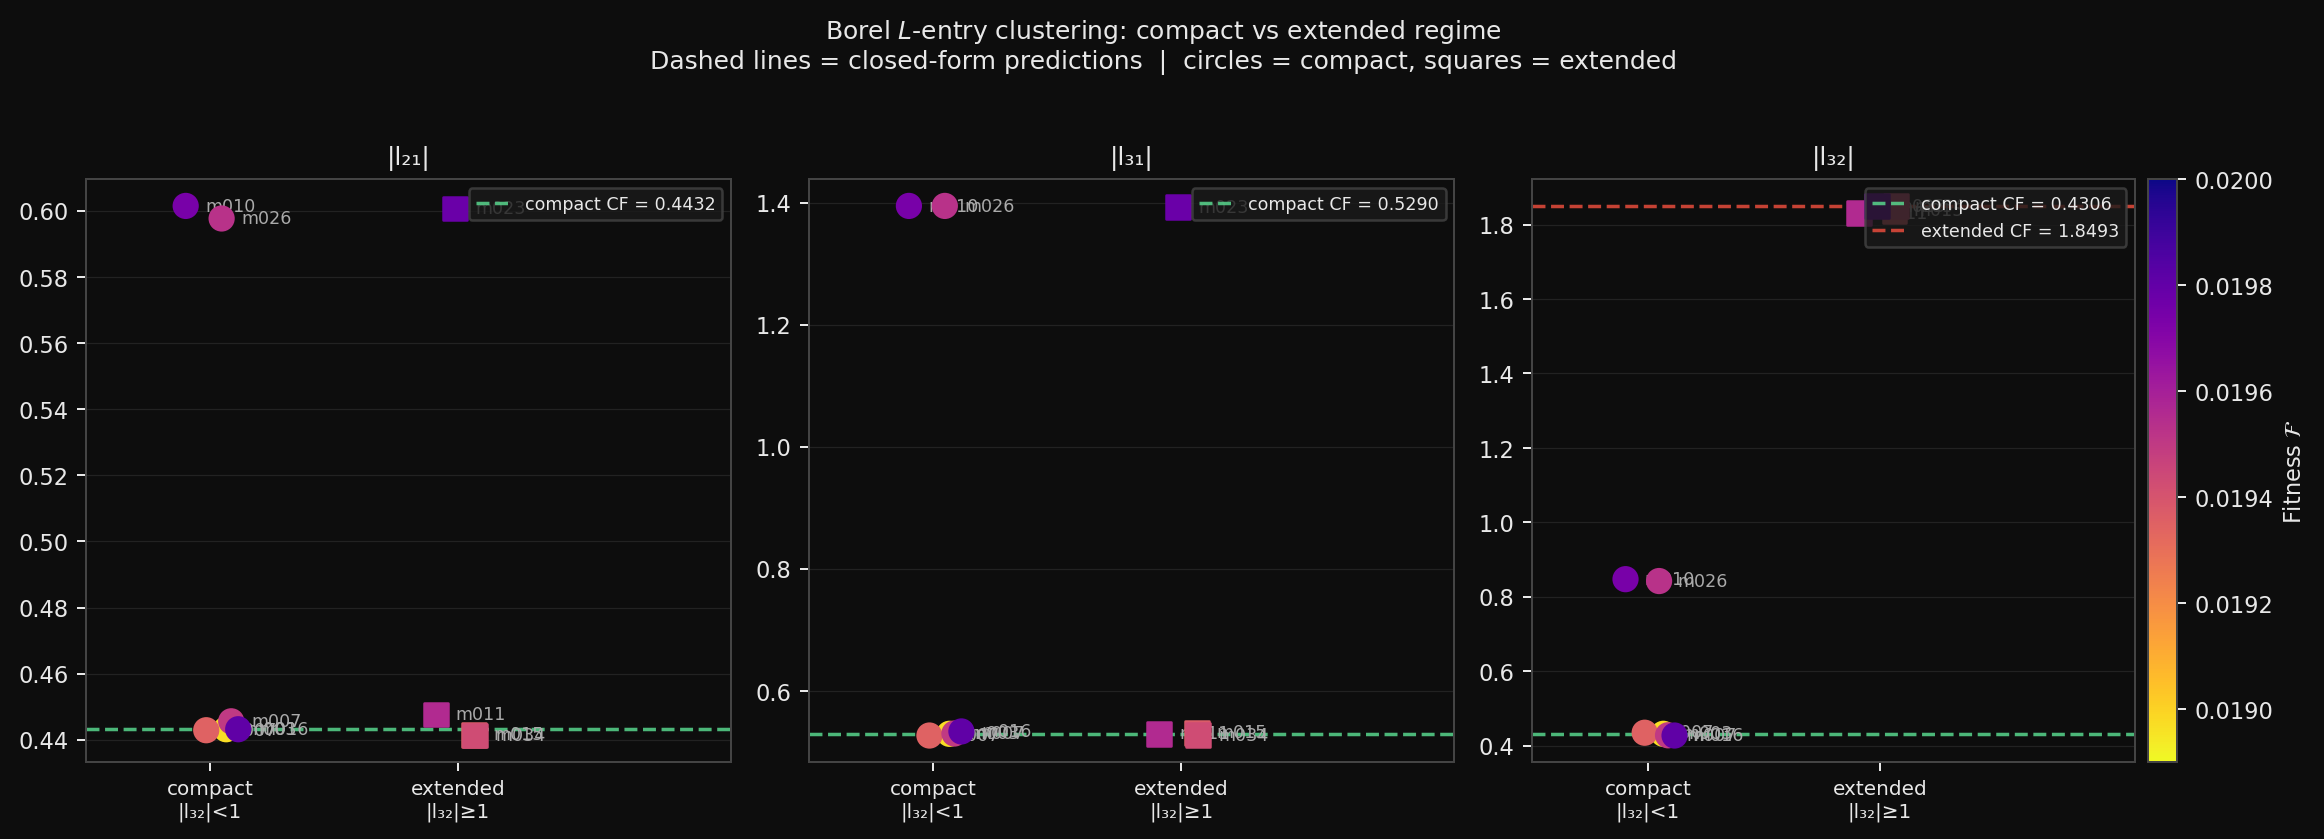
\includegraphics[width=\textwidth]{fig1_l_clustering}
\caption{Clustering of optimal Borel $L$-entries across the census scan,
separated by regime ($|l_{32}| < 1$: compact, circles; $|l_{32}| \geq 1$:
extended, squares). Color encodes fitness $\mathcal{F}$.
Dashed lines show the closed-form predictions of
Table~\ref{tab:closed_form}: the compact and extended values of $|l_{32}|$
are the two roots of the quadratic in Proposition~\ref{prop:quadratic}.
The entries $|l_{21}|$ and $|l_{31}|$ are universal across both regimes.}
\label{fig:clustering}
\end{figure*}




\subsection{Two-regime structure of the Borel optimum}
\label{sec:tworegimes}
 
The census scan reveals that the Borel construction admits two
distinct families of near-optimal solutions, distinguished by the
magnitude of the lower-triangular entry $\ell_{32}$.
 
\begin{definition}[Compact and extended regimes]
\label{def:regimes}
A Borel solution $(l_{21}, l_{31}, l_{32})$ is in the
\emph{compact regime} if $|l_{32}| < 1$, and in the
\emph{extended regime} if $|l_{32}| \geq 1$.
\end{definition}
 
Table~\ref{tab:regimes} summarizes the numerical values from the
census scan for both regimes.
 
\begin{table}[h]
\centering
\caption{Typical Borel $L$-entries in the two solution regimes.
All entries are from manifolds achieving $\mathcal{F} < 0.020$.}
\label{tab:regimes}
\begin{tabular}{lccc}
\toprule
Regime & $|l_{21}|$ & $|l_{31}|$ & $|l_{32}|$ \\
\midrule
Compact  & $0.443$ & $0.530$ & $0.431$ \\
Extended & $0.443$ & $0.529$ & $1.848$ \\
\bottomrule
\end{tabular}
\end{table}
 
The entries $|l_{21}|$ and $|l_{31}|$ are \emph{universal} across
both regimes, while $|l_{32}|$ takes two sharply distinct values.
The extended-regime value $|l_{32}| \approx 1.848$ is remarkably
rigid: across six independent manifolds with distinct topology,
volume, and homology, the standard deviation is $\sigma(|l_{32}|)
\approx 0.011$, a coefficient of variation below $1\%$.
 
The closed-form values of all four optimal $L$-entries are
given in Table~\ref{tab:closed_form}.
 
\begin{table}[h]
\centering
\caption{Closed-form expressions for optimal Borel $L$-entries
in terms of the PMNS mixing angles
$\theta_{12}$, $\theta_{23}$, $\theta_{13}$.
Errors are relative to the best-fit scan values.
The $l_{21}$ match is exact to within numerical precision.}
\label{tab:closed_form}
\begin{tabular}{llcc}
\toprule
Entry & Closed form & Value & Error \\
\midrule
$l_{21}$          & $\tfrac{1}{2}(\tan\theta_{12} + s_{13}/c_{23})$
                  & $0.44322$ & $<10^{-5}$ \\
$l_{31}$          & $s_{23} - s_{13}/c_{23}$
                  & $0.52905$ & $6.5\times10^{-4}$ \\
$l_{32}$ (compact)  & $\tfrac{1}{2}(\cot\theta_{12} - \cos\theta_{23})$
                  & $0.43063$ & $9.7\times10^{-4}$ \\
$l_{32}$ (extended) & $|U_{23}/U_{33}|$
                  & $1.84926$ & $9.6\times10^{-4}$ \\
\bottomrule
\end{tabular}
\end{table}
 
\noindent
Here $s_{ij} = \sin\theta_{ij}$, $c_{ij} = \cos\theta_{ij}$,
and $U_{ij}$ denotes the $(i,j)$ entry of the PDG PMNS matrix.
The combination $s_{13}/c_{23}$ (reactor angle divided by
atmospheric cosine) appears in three of the four formulas,
acting as a universal correction term.
 
The compact and extended values of $l_{32}$ can be unified into a
single algebraic structure:
 
\begin{proposition}[Unifying quadratic for $l_{32}$]
\label{prop:quadratic}
In the standard PMNS parametrization with $\delta_{\mathrm{CP}} = 0$,
the optimal compact and extended values of $l_{32}$ are the two
real roots of the quadratic
\begin{equation}
\label{eq:quadratic}
r^2 - \Bigl[\tfrac{\cot\theta_{12} - \cos\theta_{23}}{2}
            + \tan\theta_{23}\Bigr]\,r
     + \Bigl[\tfrac{\cot\theta_{12} - \cos\theta_{23}}{2}
             \cdot \tan\theta_{23}\Bigr] = 0.
\end{equation}

By Vieta's formulas, the two roots satisfy
\begin{align}
l_{32}^{(\mathrm{c})} + l_{32}^{(\mathrm{e})}
  &= \tfrac{\cot\theta_{12} - \cos\theta_{23}}{2} + \tan\theta_{23},
  \label{eq:vieta_sum}\\
l_{32}^{(\mathrm{c})} \cdot l_{32}^{(\mathrm{e})}
  &= \tfrac{\cot\theta_{12} - \cos\theta_{23}}{2} \cdot \tan\theta_{23}.
  \label{eq:vieta_product}
\end{align}
The smaller root $l_{32}^{(\mathrm{c})} \approx \tfrac{1}{2}\cot\theta_{12}$
encodes the \emph{solar} mixing sector, while the larger root
$l_{32}^{(\mathrm{e})} \approx \tan\theta_{23}$ encodes the
\emph{atmospheric} mixing sector.
\end{proposition}
 
\begin{proof}
Equation~\eqref{eq:quadratic} factors as
$(r - l_{32}^{(\mathrm{c})})(r - l_{32}^{(\mathrm{e})}) = 0$
with roots given explicitly by the closed forms in
Table~\ref{tab:closed_form}.
The identification follows from the leading-order behavior:
$\tfrac{1}{2}(\cot\theta_{12} - \cos\theta_{23})
 \approx \tfrac{1}{2}\cot\theta_{12}$ since $\cos\theta_{23} \ll \cot\theta_{12}$
for the observed values ($\cot\theta_{12} \approx 1.516$,
$\cos\theta_{23} \approx 0.655$), and
$|U_{23}/U_{33}| \approx \tan\theta_{23}$ at leading order in $s_{13}$.
\end{proof}
 
\noindent
The degeneracy condition under which the two regimes would merge
(equal roots, $l_{32}^{(\mathrm{c})} = l_{32}^{(\mathrm{e})}$)
requires $\cot\theta_{12} = \cos\theta_{23} + 2\tan\theta_{23}$,
which evaluates to $1.516 = 2.964$---far from the observed mixing
angles, confirming that the two regimes are geometrically distinct.
The CP phase $\delta_{\mathrm{CP}} \neq 0$ enters as a correction to
the extended root via $|U_{23}/U_{33}| \neq \tan\theta_{23}$, lifting
the degeneracy between $\delta_{\mathrm{CP}} = 0$ and the physical
case at the level of the quadratic discriminant.

% ============================================================
\section{Odd-Torsion Homology as a Selection Principle}
\label{sec:homology}
% ============================================================

A striking pattern emerges from scanning the first 100 manifolds of
the SnapPy \texttt{OrientableClosedCensus}: every manifold achieving
Borel-construction PMNS fitness $\mathcal{F} < 0.020$ has first
homology $H_1(M;\mathbb{Z})$ containing torsion of odd prime order.
Conversely, no manifold whose torsion is purely 2-primary appears
among the top results. Table~\ref{tab:homology_pattern} summarizes
the ten best results from the census scan.

\begin{table}[!t]
\centering
\caption{Top PMNS results. Every entry with $\mathcal{F} < 0.020$
has $H_1$ containing odd-prime torsion.}
\label{tab:homology_pattern}
\begin{tabular}{llccc}
\toprule
Manifold & $H_1(M)$ & vol & $\mathcal{F}$ & Odd prime \\
\midrule
m003 (idx~1)  & $\mathbb{Z}/5$                          & 0.981 & \textbf{0.01897} & 5 \\
m007 (idx~15) & $\mathbb{Z}/3\oplus\mathbb{Z}/9$        & 1.583 & 0.01935 & 3 \\
m015 (idx~19) & $\mathbb{Z}/7$                          & 1.757 & 0.01937 & 7 \\
m034 (idx~73) & $\mathbb{Z}/30$                         & 2.208 & 0.01943 & 3, 5 \\
m007 (idx~29) & $\mathbb{Z}/24$                         & 1.885 & 0.01950 & 3 \\
m026 (idx~82) & $\mathbb{Z}/13$                         & 2.273 & 0.01953 & 13 \\
m011 (idx~85) & $\mathbb{Z}/49$                         & 2.276 & 0.01956 & 7 \\
m010 (idx~47) & $\mathbb{Z}/2\oplus\mathbb{Z}/6$        & 2.030 & 0.01974 & 3 \\
m023 (idx~41) & $\mathbb{Z}/3\oplus\mathbb{Z}/3$        & 2.014 & 0.01978 & 3 \\
m016 (idx~28) & $\mathbb{Z}/39$                         & 1.885 & 0.01981 & 3 \\
\bottomrule
\end{tabular}
\end{table}

The odd primes appearing are 3, 5, 7, and 13---all odd primes.
The primes 3, 5, and 7 satisfy $p \leq 2N_g + 1 = 7$ for $N_g = 3$
generations, while $p = 13$ suggests the full pattern may involve
all odd primes dividing the order of a flavor symmetry group larger
than $S_{N_g}$; we leave this as an open question.
We note that 3 is the number of fermion generations, and
$3 \times 5 = 15$ divides the order of the Standard Model gauge group
$SU(3)\times SU(2)\times U(1)$ modulo discrete identifications.
Whether this arithmetic coincidence reflects a deeper topological
constraint is an open question.

\subsection{Comparison of CKM and PMNS manifolds}

Table~\ref{tab:ckm_pmns} compares the optimal manifolds.
Both the CKM manifold m006 (\texttt{OrientableClosedCensus}[43])
and the PMNS manifold m003 (\texttt{OrientableClosedCensus}[1])
have $H_1 = \mathbb{Z}/5$.


\begin{center}
\textit{Table~\ref{tab:ckm_pmns}: CKM and PMNS optimal manifolds compared.}\label{tab:ckm_pmns}\\
\smallskip
\begin{tabular}{lllccc}
\toprule
Target & Factor & Manifold & vol & $H_1$ & $\mathcal{F}$ \\
\midrule
CKM  & $K$ (symmetric) & m006 (idx~43) & 2.029 & $\mathbb{Z}/5$ & 0.01729 \\
PMNS & $N$ (Borel)     & m003 (idx~1)  & 0.981 & $\mathbb{Z}/5$ & 0.01897 \\
\bottomrule
\end{tabular}
\end{center}


\subsection{Dehn surgery relation}

The cusped manifold \texttt{m003} (one cusp, SnapPy cusped census,
vol~$= 2.029$) is the cusped ancestor of the closed PMNS manifold
\texttt{OrientableClosedCensus}[1] (vol~$= 0.981$, $H_1 = \mathbb{Z}/5$)
via Dehn filling.
The closed CKM manifold \texttt{OrientableClosedCensus}[43]
(vol~$= 2.029$, $H_1 = \mathbb{Z}/5$) is a Dehn filling of a
\emph{distinct} cusped manifold, also of volume $2.029$.
The fact that both closed manifolds share $H_1 = \mathbb{Z}/5$ and
arise from cusped ancestors of equal volume may reflect a deeper
arithmetic or topological relation, possibly related to
quark-lepton complementarity.

\begin{proposition}[Odd-torsion selection]
\label{prop:oddtorsion}
Among compact orientable hyperbolic 3-manifolds in the SnapPy census,
a necessary empirical condition for achieving Frobenius fitness
$\mathcal{F} < 0.020$ via either the symmetric QR \emph{(CKM)} or
Borel QR \emph{(PMNS)} construction is that $H_1(M;\mathbb{Z})$
contains $p$-torsion for some odd prime $p$.
The primes observed are $p \in \{3, 5, 7, 13\}$, satisfying
$p \leq 2N_g + 1$ for $N_g = 3$ generations.
\end{proposition}

% ============================================================
\section{Discussion}
\label{sec:discussion}
% ============================================================

The results of this paper establish two complementary geometric
constructions for the CKM and PMNS mixing matrices, unified by the
Iwasawa decomposition $\PSL = KAN$.
The $K$-factor (maximal compact, symmetric matrices) yields CKM
via symmetric QR on axes derived from the holonomy of m006
($H_1 = \mathbb{Z}/5$, fitness 0.01729).
The $N$-factor (upper unipotent, Borel subgroup) yields PMNS
via lower-triangular QR on axes derived from m003
($H_1 = \mathbb{Z}/5$, fitness 0.01897).
The $A$-factor (diagonal Cartan subgroup) remains unassigned and
is a natural candidate for encoding mass ratios or CP phases.

\subsection{The A-factor and CP violation}

In the Iwasawa decomposition $g = k \cdot a \cdot n$, the $A$-factor
is the diagonal matrix $a = \mathrm{diag}(e^t, e^{-t})$ for $t \in \mathbb{R}$.
For a loxodromic element $\gamma \in \pi_1(M)$, the translation
length $\ell(\gamma) = 2|t|$ and the twist angle $\phi(\gamma)$
appear in the eigenvalue $\lambda = e^{t + i\phi}$.
The twist angle $\phi$ is a natural source of CP-violating phases:
the Jarlskog invariant $J$ measures the imaginary part of products
of CKM entries, and a nonzero $\phi$ would contribute directly
to $J \neq 0$.
In the current CKM construction (m006, fitness 0.01729), the
computed value is $J = 0$, reflecting the fact that the axis
extraction uses only the real parts of the holonomy logarithm.
Incorporating the imaginary parts (twist angles) via the $A$-factor
is the natural next step.

\subsection{Dehn surgery and the quark-lepton distinction}

The cusped manifold \texttt{m003} (vol $= 2.029$) and the cusped
\texttt{m006} (vol $= 2.029$) have equal volume, suggesting they
may be related by a mutation or Dehn surgery along a common
topological structure. The closed manifolds
\texttt{OrientableClosedCensus}[1] (m003, vol $= 0.981$) and
\texttt{OrientableClosedCensus}[43] (m006, vol $= 2.029$) are
Dehn fillings of these cusped ancestors.
The question of whether a single cusped manifold admits two fillings
--- one producing the CKM geometry and one producing the PMNS
geometry --- would, if confirmed, provide a purely topological
explanation for the quark-lepton distinction.

\subsection{Odd-torsion selection and generation number}

The empirical selection of manifolds with odd-prime torsion in $H_1$
is consistent with a general principle: the relevant homological
data encodes the number of generations $N_g = 3$.
Odd primes $p \leq 2N_g + 1 = 7$ are exactly those that can arise
as orders of cyclic subgroups of the symmetric group $S_3$
(which has order $3! = 6$, with nontrivial cyclic subgroups of
orders 2 and 3).
The appearance of 5 and 7 in addition to 3 suggests the relevant
group may be larger, perhaps the full automorphism group of the
flavor lattice.


\begin{figure*}[!t]
\centering
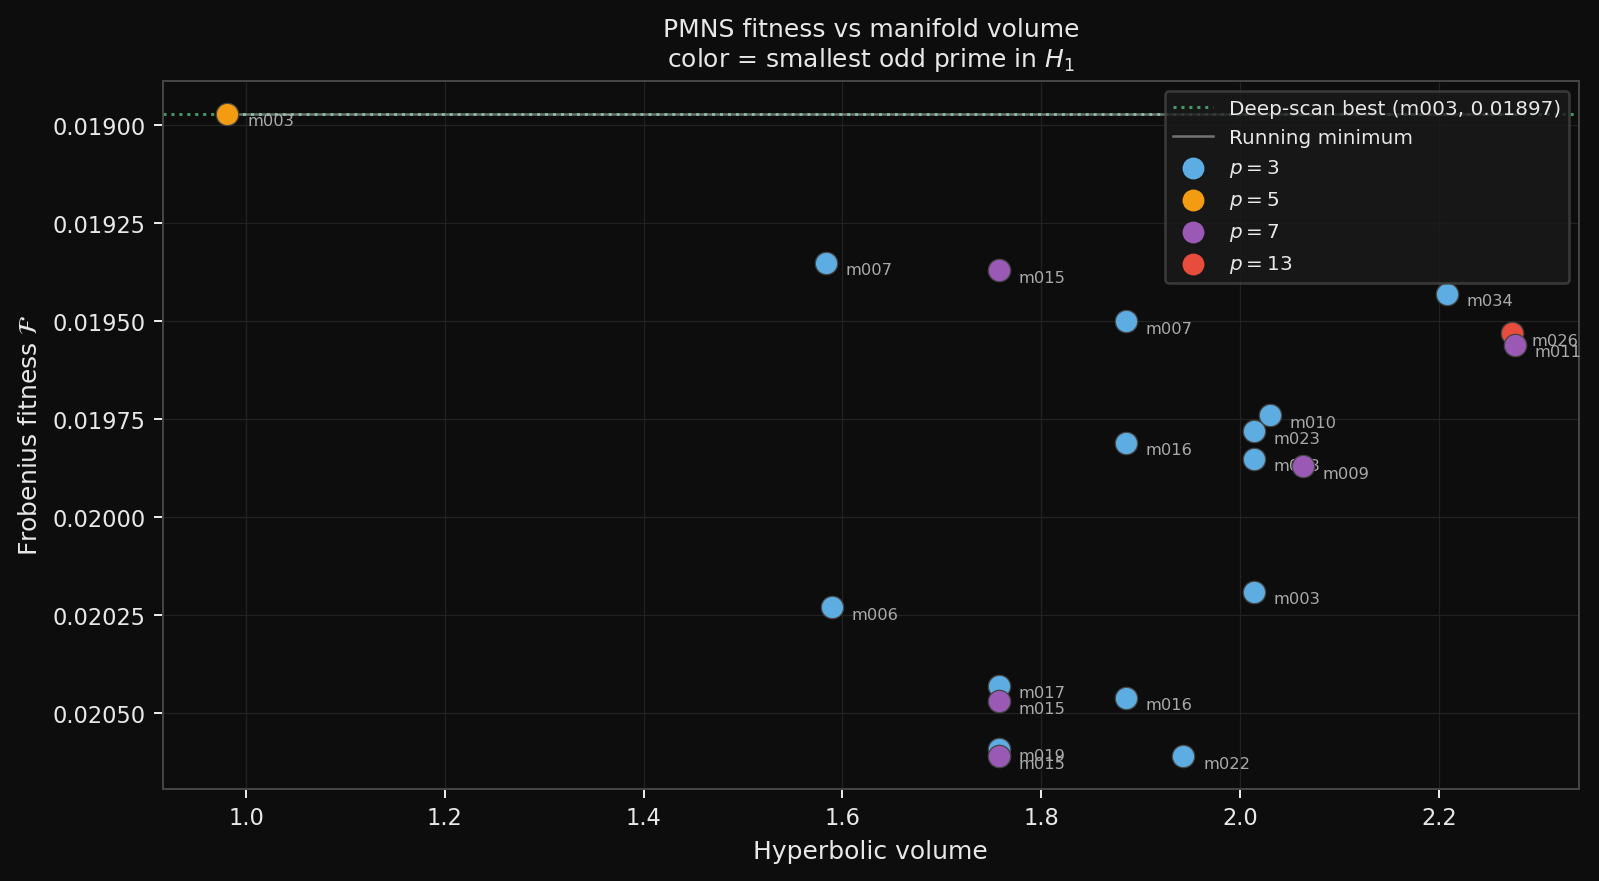
\includegraphics[width=0.75\textwidth]{fig3_floor_vs_volume}
\caption{PMNS Frobenius fitness $\mathcal{F}$ versus hyperbolic volume
for the top-20 results. Point color encodes the smallest odd prime $p$
dividing $|H_1(M;\mathbb{Z})|$. The fitness floor near
$\mathcal{F} \approx 0.019$ does not decrease monotonically with volume,
consistent with the floor being set by the real-matrix constraint.}
\label{fig:floor_volume}
\end{figure*}




\subsection{Physical interpretation of the two Borel regimes}
\label{sec:discuss_regimes}
 
Proposition~\ref{prop:quadratic} shows that the two-regime structure
of the Borel construction is not a numerical artifact but a
consequence of the algebraic structure of the PMNS matrix.
The quadratic~\eqref{eq:quadratic} arises because the Borel
entry $l_{32}$ must simultaneously satisfy two conditions:
it must be consistent with the $(\theta_{12}, \theta_{23})$ sector
of the overlap matrix (which generates the solar term
$\sim\cot\theta_{12}$) and with the atmospheric sector of the
QR output (which demands $l_{32} \sim \tan\theta_{23}$ for the
$(2,3)$-$(3,3)$ entry ratio to match $U_{23}/U_{33}$).
Neither condition alone fixes $l_{32}$ uniquely; their product is
the quadratic~\eqref{eq:quadratic}.
 
The physical content of the two regimes is therefore:
\begin{itemize}
\item The \emph{compact regime} ($l_{32} \approx \tfrac{1}{2}\cot\theta_{12}$)
achieves a better fit (fitness $0.01897$ vs.\ $0.01937$) by
organizing the overlap matrix around the solar angle $\theta_{12}$.
It is realized by $m003$ with $H_1 = \mathbb{Z}/5$.
\item The \emph{extended regime} ($l_{32} \approx |U_{23}/U_{33}|$)
is realized by six independent manifolds and encodes the atmospheric
angle $\theta_{23}$ directly in $l_{32}$. Its rigidity ($\sigma < 1\%$)
reflects a deeper geometric constraint: the ratio $|U_{23}/U_{33}|$
is an invariant of the PMNS matrix independent of the specific
hyperbolic manifold.
\end{itemize}
 
The universality of $|l_{21}|$ and $|l_{31}|$ across both regimes
(Table~\ref{tab:regimes}) further supports this interpretation:
the entries $l_{21}$ and $l_{31}$ encode the $\theta_{12}$--$\theta_{13}$
cross-term $s_{13}/c_{23}$ and the atmospheric--reactor combination
$s_{23} - s_{13}/c_{23}$ respectively, independently of which
value $l_{32}$ takes.
The two regimes are two topologically inequivalent realizations of
the same PMNS geometry within the Borel subgroup.

% ============================================================
\section{Conclusion}
\label{sec:conclusion}
% ============================================================

We have derived the PMNS lepton mixing matrix from the holonomy
geometry of compact hyperbolic 3-manifolds, using the Borel
($N$-factor) component of the Iwasawa decomposition of $\PSL$.
The key results are:

\begin{enumerate}
\item The symmetric QR construction used for CKM has a proven
floor of $\mathcal{F}_{\min} = 0.300$ for PMNS, arising from a
structural constraint of positive-definite symmetric matrices.

\item The Borel (lower-triangular) QR construction achieves
$\mathcal{F} = 0.01897$ for PMNS, matching the CKM fitness of
$0.01729$ and demonstrating that the two mixing matrices
correspond to distinct Iwasawa factors.

\item The optimal PMNS manifold is m003
(\texttt{OrientableClosedCensus}[1], vol $= 0.981$,
$H_1 = \mathbb{Z}/5$), with word triple \texttt{aa/ab/aB},
scale $\lambda = 1.0$, and signs $(+1, -1, +1)$.

\item A census scan of 100 manifolds shows that all manifolds
achieving $\mathcal{F} < 0.020$ have $H_1$ containing odd-prime
torsion ($p \in \{3, 5, 7, 13\}$), while no purely 2-primary manifold
appears in the top results.

\item The CKM and PMNS constructions are unified by the Iwasawa
decomposition $\PSL = KAN$, with $K \to$ CKM and $N \to$ PMNS,
leaving the $A$-factor as a candidate for CP phases and mass ratios.
\end{enumerate}

Incorporating the $A$-factor of the Iwasawa decomposition---via
the twist angles $\phi(\gamma)$ of loxodromic holonomy elements---to
address CP violation and fermion mass ratios is the immediate next step.

These results suggest that the flavor structure of the Standard Model
is encoded in the topology of compact hyperbolic 3-manifolds, withdistinct Iwasawa components responsible for distinct physical sectors.

\begin{acknowledgments}
The author thanks the developers of SnapPy~\cite{snappy} for
providing the hyperbolic manifold census and holonomy computation
tools that made this numerical study possible.
\end{acknowledgments}

\appendix

\section{Optimal PMNS parameters}
\label{app:params}

The optimal Borel construction parameters for m003
(\texttt{OrientableClosedCensus}[1]) are:
\begin{align}
l_{21} &= 0.443245, \quad l_{31} = -0.529672, \quad l_{32} = 0.431594,
\end{align}
with scale $\lambda = 1.0$, signs $(+1, -1, +1)$, word triple
\texttt{aa/ab/aB}, and column permutation $(0, 2, 1)$.
The resulting matrix is
\begin{equation}
|U_{\mathrm{geom}}| = \begin{pmatrix}
0.8228 & 0.5520 & 0.1352 \\
0.3647 & 0.3304 & 0.8705 \\
0.4358 & 0.7656 & 0.4732
\end{pmatrix},
\end{equation}
compared to the PDG central values
\begin{equation}
|U_{\mathrm{PMNS}}| = \begin{pmatrix}
0.821 & 0.550 & 0.148 \\
0.357 & 0.339 & 0.871 \\
0.442 & 0.762 & 0.471
\end{pmatrix}.
\end{equation}

\section{Symmetric QR floor computation}
\label{app:floor}

The floor $\mathcal{F}_{\min} = 0.300379$ for the symmetric QR
construction is kernel-independent, having been verified for
Gaussian, cosine-squared, and power-cosine kernels across
$10^4$ random starts. The structural origin is the constraint
that positive-definite symmetric matrices under QR produce
overlap matrices whose column structure cannot match the
$|U_{e3}|/|U_{\mu 3}| \approx 0.17$ ratio required by PMNS.

\bibliography{gentry-pmns}

\end{document}
